\documentclass[11pt,a4paper]{article}
\usepackage[utf8]{inputenc}
\usepackage[T1]{fontenc}
\usepackage{lmodern}
\usepackage[margin=2.5cm]{geometry}
\usepackage{booktabs}
\usepackage{graphicx}
\usepackage{caption}
\usepackage{float}
\usepackage{amsmath}
\usepackage{breqn}
\usepackage[hidelinks]{hyperref}

\title{An automatic report for the dataset: airline passengers}
\author{Some Math empowered by some AI guided by some researchers}
\date{09 November 2026}

\begin{document}
\maketitle

\noindent\emph{Produced by \texttt{autostat}, a Python 3 port of the Automatic Bayesian Covariance Discovery system of Lloyd et al. (AAAI 2014).}


\begin{figure}[H]
\centering
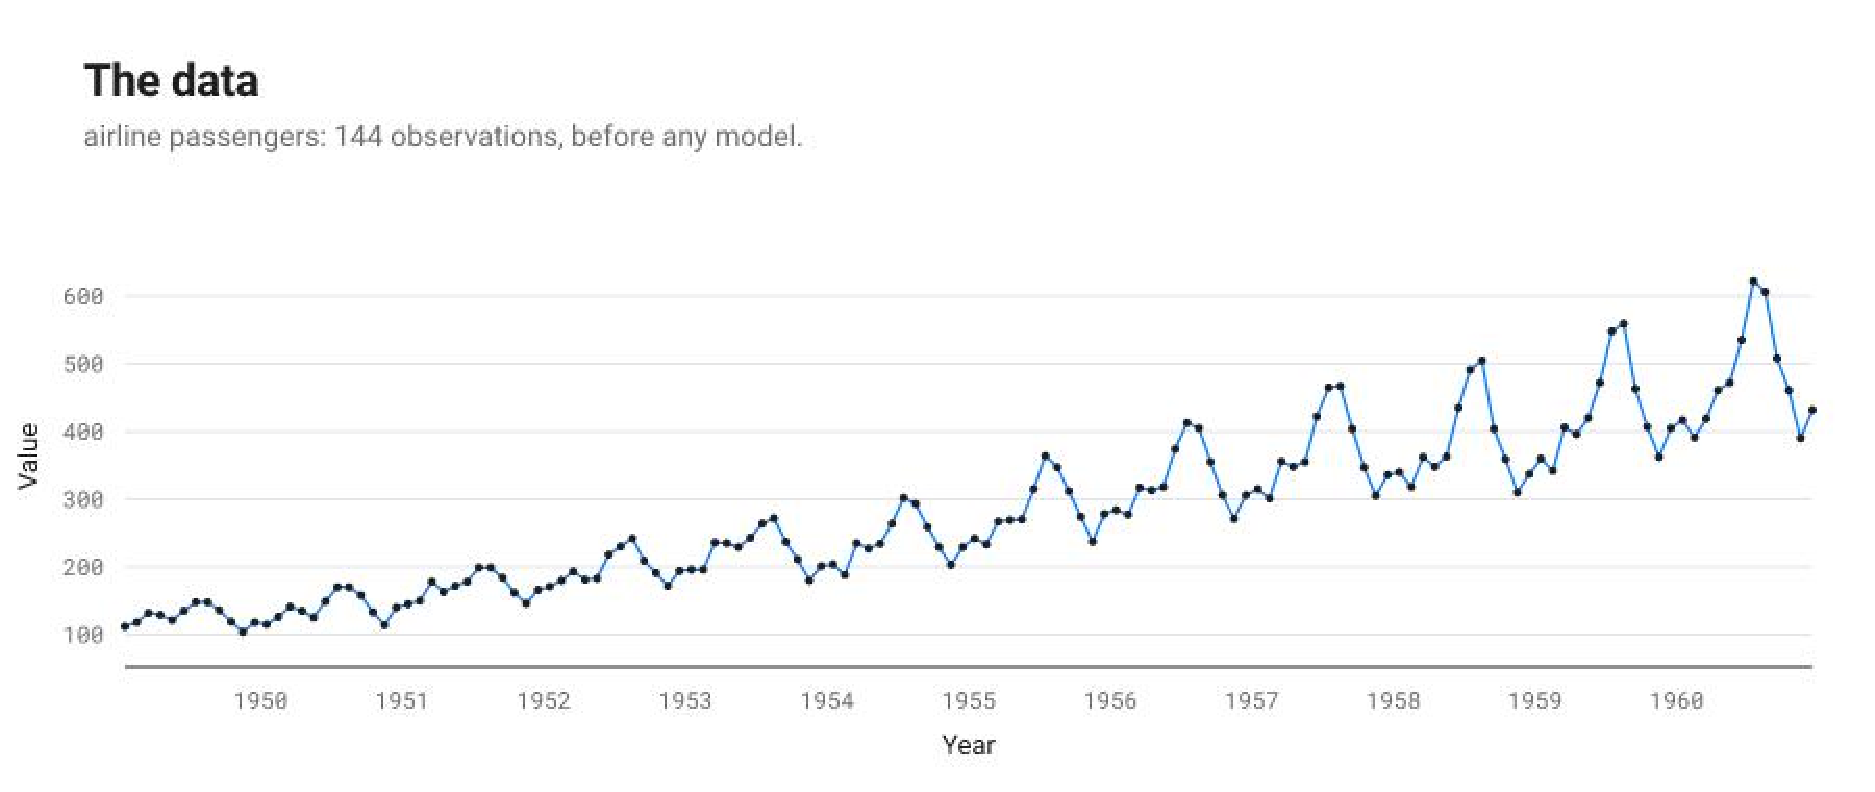
\includegraphics[width=\linewidth]{data.pdf}
\caption*{The data}
\end{figure}

\section*{Executive summary}

The structure search selected \texttt{Lin x Per + (Lin + RQ) x (Lin + Lin x Per)} (Bayesian information criterion 1112.4; negative log likelihood 521.4 on 144 points). It decomposes into 5 additive components, listed by how much each reduces extrapolation error:
\begin{enumerate}
  \item A quadratic polynomial.
  \item This simple AI is not capable of describing the component Lin x RQ.
  \item A periodic function with a period of 1.0 years but with quadraticly varying amplitude.
  \item This simple AI is not capable of describing the component Lin x Per x RQ.
  \item A periodic function with a period of 4.2 years but with linearly increasing amplitude.
\end{enumerate}

\begin{center}
\begin{tabular}{lrrrr}
\toprule
\# & $R^2$ cumulative (\%) & Residual variance explained (\%) & CV MAE & MAE reduction (\%) \\
\midrule
data & & & 280 & \\
1 & 81.6 & 81.6 & 106 & 62.1 \\
2 & 86.6 & 27.1 & 32.3 & 69.5 \\
3 & 97.1 & 78.6 & 16.5 & 48.9 \\
4 & 99.6 & 87.3 & 8.57 & 48.1 \\
5 & 100.0 & 100.0 & 5.84 & 31.9 \\
\bottomrule
\end{tabular}
\end{center}

MAE: mean absolute error over ten contiguous held-out blocks; CV: cross-validated.

\section*{The formula found}

The structure search is a symbolic regression: it searches a grammar of expressions over kernels and keeps the one with the lowest Bayesian information criterion. This is the expression it kept, with every fitted parameter in place; $t$ is in years.
\begin{dmath*}
y(t) = f_{1}(t) + f_{2}(t) + f_{3}(t) + f_{4}(t) + f_{5}(t) + \varepsilon(t)
\end{dmath*}

Each component is a Gaussian process with its own covariance:
\begin{dmath*}
f_{1}(t) \sim \mathrm{GP}\!\left(0,\ 0.7107\,(t - 1943)(t' - 1943) \cdot (t - 1940)(t' - 1940)\right)
\end{dmath*}
\begin{dmath*}
f_{2}(t) \sim \mathrm{GP}\!\left(0,\ 56.66\,(t - 1940)(t' - 1940) \cdot \left(1 + \frac{(t - t')^2}{2 \cdot 1.654 \times 10^{-4} \cdot 0.001875^2}\right)^{-1.654 \times 10^{-4}}\right)
\end{dmath*}
\begin{dmath*}
f_{3}(t) \sim \mathrm{GP}\!\left(0,\ 0.04947\,(t - 1943)(t' - 1943) \cdot (t - 1944)(t' - 1944) \cdot \frac{\exp\!\left(2.195\cos\frac{2\pi (t - t')}{1.002}\right) - I_0(2.195)}{e^{2.195} - I_0(2.195)}\right)
\end{dmath*}
\begin{dmath*}
f_{4}(t) \sim \mathrm{GP}\!\left(0,\ 3.944\,(t - 1944)(t' - 1944) \cdot \frac{\exp\!\left(2.195\cos\frac{2\pi (t - t')}{1.002}\right) - I_0(2.195)}{e^{2.195} - I_0(2.195)} \cdot \left(1 + \frac{(t - t')^2}{2 \cdot 1.654 \times 10^{-4} \cdot 0.001875^2}\right)^{-1.654 \times 10^{-4}}\right)
\end{dmath*}
\begin{dmath*}
f_{5}(t) \sim \mathrm{GP}\!\left(0,\ 0.4332\,(t - 1943)(t' - 1943) \cdot \frac{\exp\!\left(1.132\cos\frac{2\pi (t - t')}{4.18}\right) - I_0(1.132)}{e^{1.132} - I_0(1.132)}\right)
\end{dmath*}
\begin{dmath*}
\varepsilon(t) \sim \mathrm{N}\!\left(0,\ 1.091 \times 10^{-10}\right)
\end{dmath*}

These components have a closed form, read from their posterior mean:
\begin{dmath*}
f_{1}(t) = 48.88 + 13.61\,(t - 1949) + 0.9081\,(t - 1949)^{2}
\end{dmath*}

The other components are smooth, quasi-periodic or noise without a short formula: a draw from such a process has no finite closed form; its covariance above is the formula.

Closed form of each component:

\begin{center}\footnotesize
\begin{tabular}{lp{0.36\linewidth}l}
\toprule
\# & component & closed form \\
\midrule
1 & A quadratic polynomial & exact polynomial of degree 2 \\
2 & This simple AI is not capable of describing the component Lin x RQ & none: the covariance is the formula \\
3 & A periodic function with a period of 1.0 years but with quadraticly varying amplitude & none: the covariance is the formula \\
4 & This simple AI is not capable of describing the component Lin x Per x RQ & none: the covariance is the formula \\
5 & A periodic function with a period of 4.2 years but with linearly increasing amplitude & none: the covariance is the formula \\
\bottomrule
\end{tabular}
\end{center}

\section*{Search path and stopping criterion}

The 2014 configuration searches a fixed number of levels and keeps the lowest BIC; it has no stopping rule. The table follows the winner of each level. A change of structure adds or removes terms; a level that keeps the structure only refits its parameters. BIC differences read on the scale of Kass and Raftery (1995): under 2 barely worth mentioning, 2 to 6 positive, 6 to 10 strong, over 10 very strong.

\begin{center}\footnotesize
\begin{tabular}{lllp{0.36\linewidth}lll}
\toprule
level & BIC & change & structure & components & closed & params \\
\midrule
1 & 1513.7 &  & RQ & 1 & 0 & 3 \\
2 & 1398.4 & -115.3 & Lin + RQ & 2 & 1 & 5 \\
3 & 1370.4 & -28.0 & Lin x RQ + RQ & 2 & 0 & 7 \\
4 & 1323.2 & -47.2 & (Lin + Per) x RQ + RQ & 3 & 0 & 10 \\
5 & 1177.0 & -146.1 & (Lin + Per x RQ) x RQ + RQ & 3 & 0 & 12 \\
6 & 1141.8 & -35.3 & (Lin + Per x RQ) x (Lin + RQ) + RQ & 5 & 1 & 14 \\
7 & 1128.3 & -13.5 & (Lin + Lin x Per) x (Lin + RQ) + RQ & 5 & 1 & 13 \\
8 & 1118.0 & -10.3 & (Lin + Lin x Per) x (Lin + RQ) + C & 5 & 2 & 11 \\
9 & 1112.7 & -5.3 & (Lin + Lin x Per) x (Lin + RQ) + Per & 5 & 2 & 13 \\
10 & 1112.4 & -0.2 & (Lin + Lin x Per) x (Lin + RQ) + Lin x Per & 5 & 1 & 14 \\
11 & 1112.4 & -0.0 & (Lin + Lin x Per) x (Lin + RQ) + Lin x Per & 5 & 1 & 14 \\
12 (kept) & 1112.4 & -0.0 & (Lin + Lin x Per) x (Lin + RQ) + Lin x Per & 5 & 1 & 14 \\
\bottomrule
\end{tabular}
\end{center}

\begin{figure}[H]
\centering
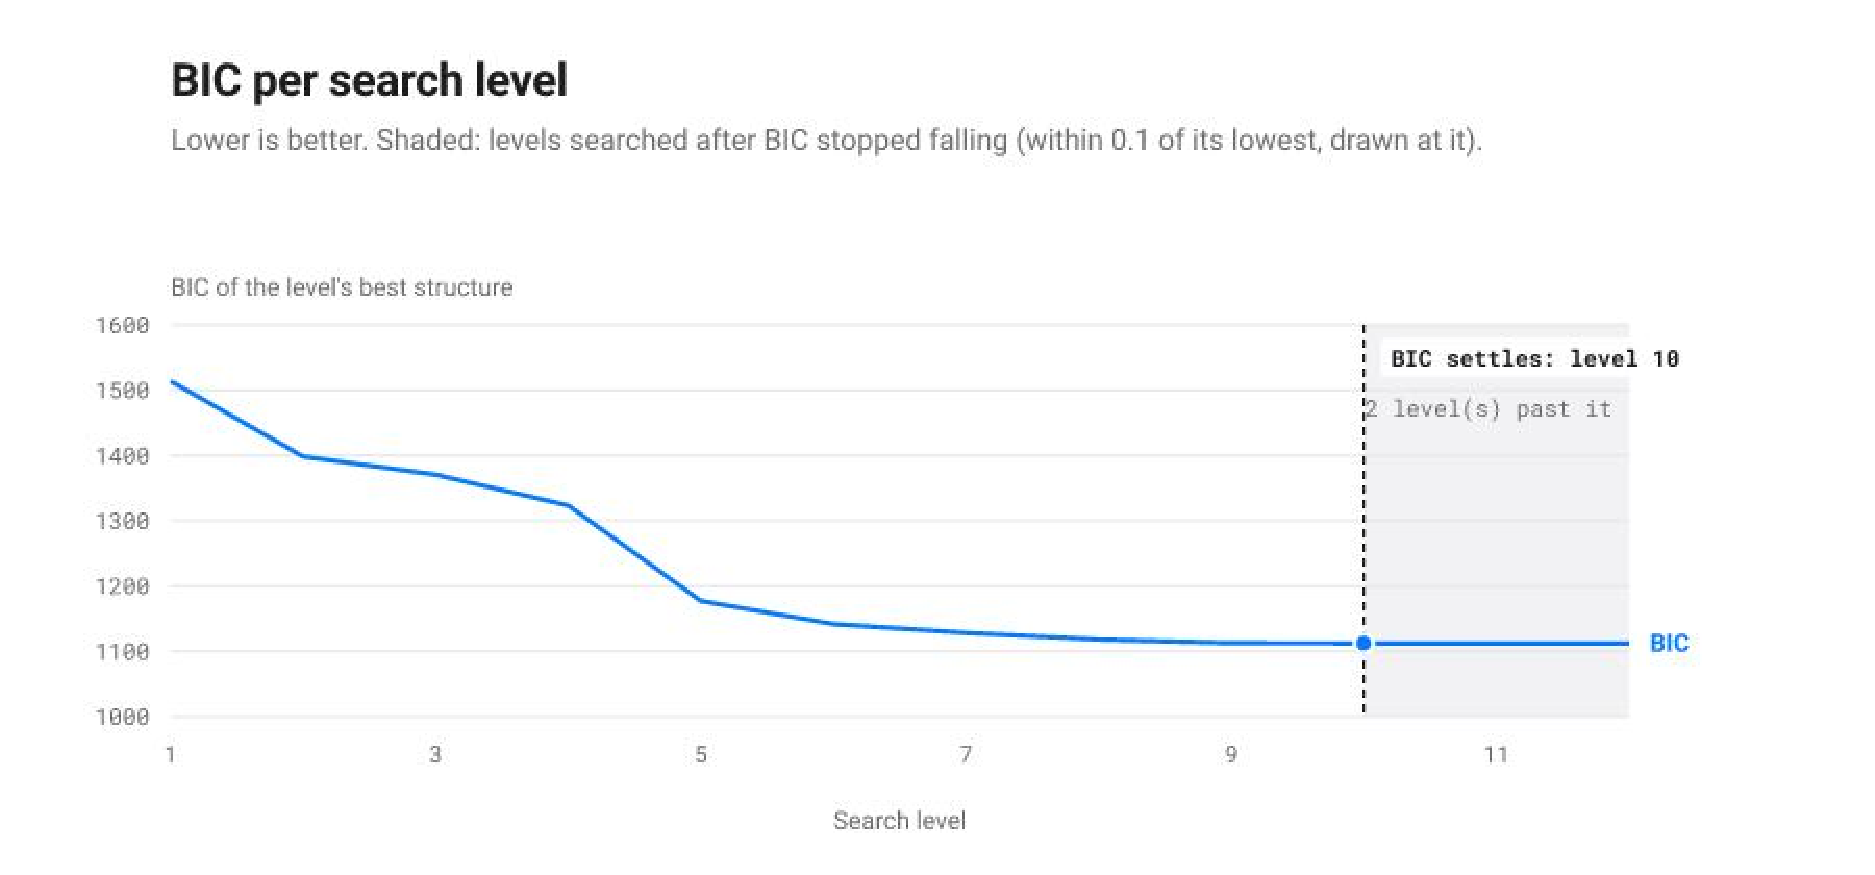
\includegraphics[width=\linewidth]{bic.pdf}
\caption*{BIC per search level}
\end{figure}

Posterior weight of each structure met, exp(-BIC/2) normalised under a flat prior, after the Bayesian machine scientist (Guimerà et al., 2020): where the search keeps one structure, the weights say how much the data prefer it to the others. The 7 structure(s) under 0.001 are left out.

\begin{center}\footnotesize
\begin{tabular}{p{0.36\linewidth}ll}
\toprule
structure & lowest BIC & weight \\
\midrule
(Lin + Lin x Per) x (Lin + RQ) + Lin x Per & 1112.4 & 0.513 \\
(Lin + Lin x Per) x (Lin + RQ) + Per & 1112.7 & 0.455 \\
(Lin + Lin x Per) x (Lin + RQ) + C & 1118.0 & 0.032 \\
\bottomrule
\end{tabular}
\end{center}

\begin{itemize}
\item The search ran 12 levels (stopping after 2 level(s) without a BIC fall above 0.1, at most 20) and keeps the model of level 12, (Lin + Lin x Per) x (Lin + RQ) + Lin x Per, BIC 1112.4.
\item That structure was first reached at level 10; the levels after it only refitted its parameters, lowering BIC by 0.0 in all.
\item The best different structure, (Lin + Lin x Per) x (Lin + RQ) + Per (level 9), is 0.2 above it: barely worth mentioning evidence for the kept one on the Kass and Raftery scale.
\item Weighed by exp(-BIC/2) under a flat prior, as the Bayesian machine scientist weighs expressions, the structures met give the kept one a posterior weight of 0.513 and the next, (Lin + Lin x Per) x (Lin + RQ) + Per, 0.455: the data barely tell them apart.
\item BIC stopped falling at level 10. The 2 level(s) searched past it kept its structure and lowered BIC by 0.00 in all, less than the tolerance of 0.1: going on buys nothing the data pay for.
\item A rule stopping after 1 level(s) without a fall above 0.1 would have ended the search at level 11 and kept the same structure, less refitted.
\item A rule stopping after 2 level(s) without a fall above 0.1 would have ended the search at level 12 and kept the same model.
\item The kept expression has 14 parameters for 144 points: its BIC is a fit term 2 NLL = 1042.9 plus a complexity term p ln n = 69.6, each extra parameter costing 4.97; it splits into 5 components, 1 of them with a closed form.
\end{itemize}

\begin{figure}[H]
\centering
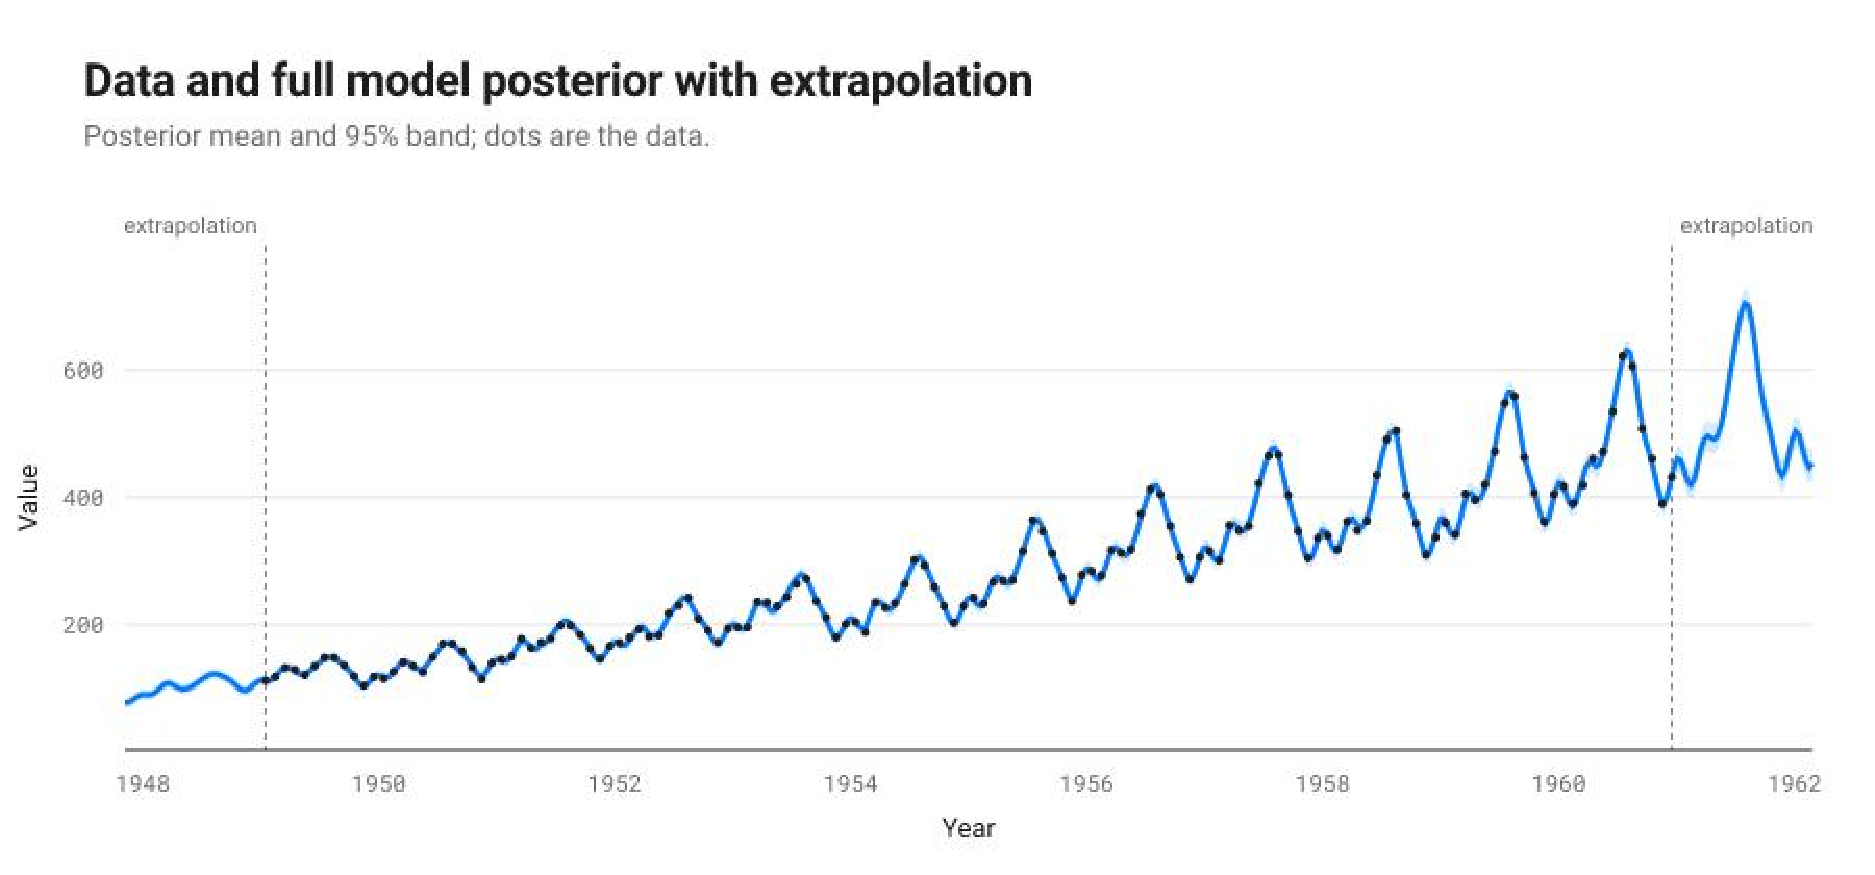
\includegraphics[width=\linewidth]{fit.pdf}
\caption*{Data and full posterior}
\end{figure}

\section*{Detailed discussion of the components}

\subsection*{Component 1: A quadratic polynomial}

This component is a quadratic polynomial.

This component explains 81.6\% of the data's variance on its own; with the components above it, 81.6\%. Adding it changes the cross-validated MAE by -62.1\%.

\emph{Extrapolation.} This component is assumed to continue as a quadratic polynomial.

\begin{figure}[H]
\centering
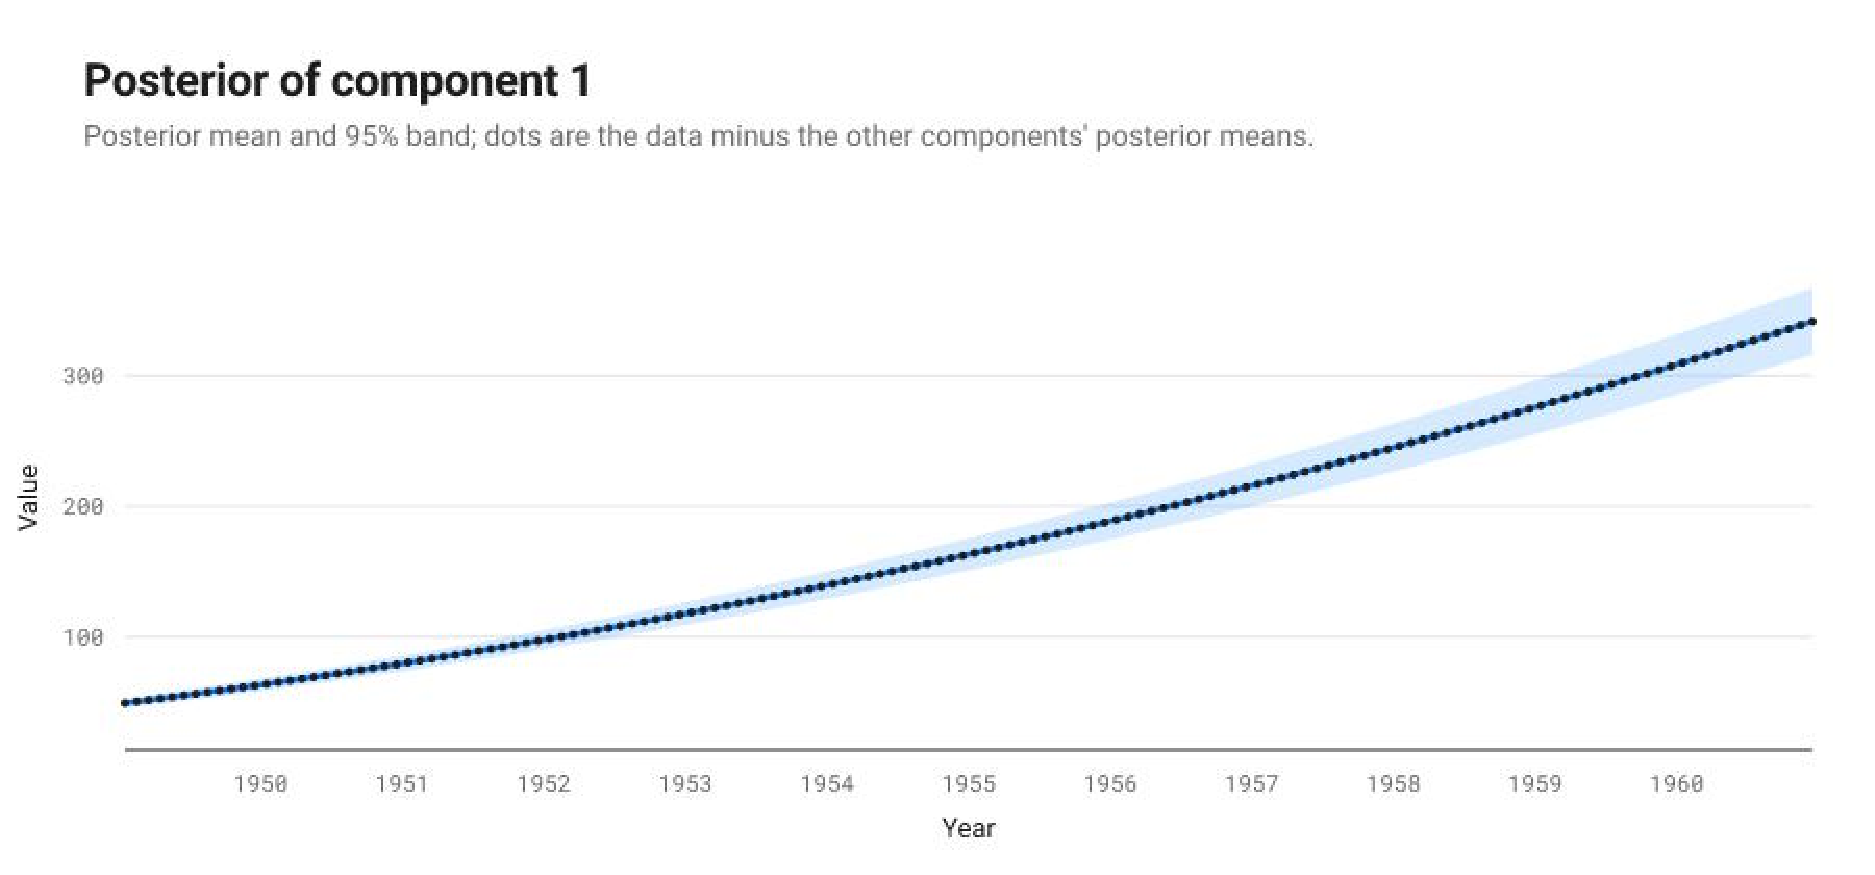
\includegraphics[width=\linewidth]{component_1.pdf}
\caption*{Component 1}
\end{figure}
\subsection*{Component 2: This simple AI is not capable of describing the component Lin x RQ}

This simple AI is not capable of describing the component Lin x RQ.

This component explains 35.3\% of the data's variance on its own; with the components above it, 86.6\%. Adding it changes the cross-validated MAE by -69.5\%.

\emph{Extrapolation.} This simple AI is not capable of describing the component Lin x RQ.

\begin{figure}[H]
\centering
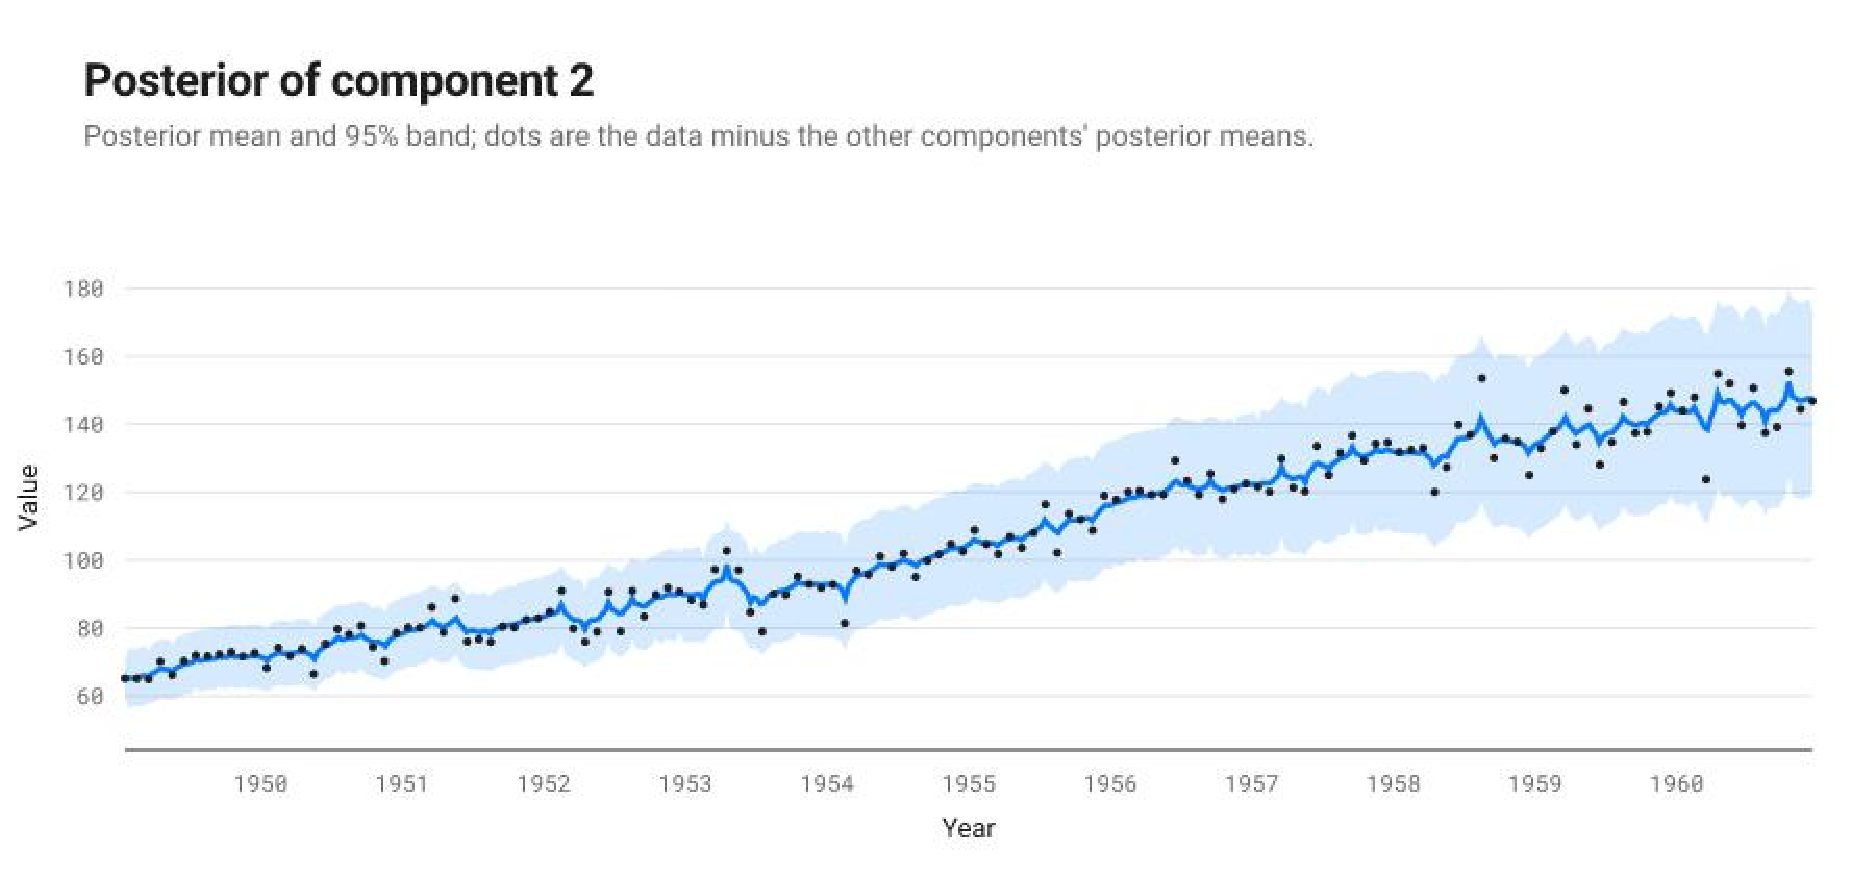
\includegraphics[width=\linewidth]{component_2.pdf}
\caption*{Component 2}
\end{figure}
\subsection*{Component 3: A periodic function with a period of 1.0 years but with quadraticly varying amplitude}

This component is periodic with a period of 1.0 years but with varying amplitude. The amplitude of the function varies quadraticly. The shape of this function within each period has a typical lengthscale of 5.6 weeks.

This component explains 11.9\% of the data's variance on its own; with the components above it, 97.1\%. Adding it changes the cross-validated MAE by -48.9\%.

\emph{Extrapolation.} This component is assumed to continue periodically with a period of 1.0 years but with varying amplitude. The amplitude of the function is assumed to continue to vary quadraticly.

\begin{figure}[H]
\centering
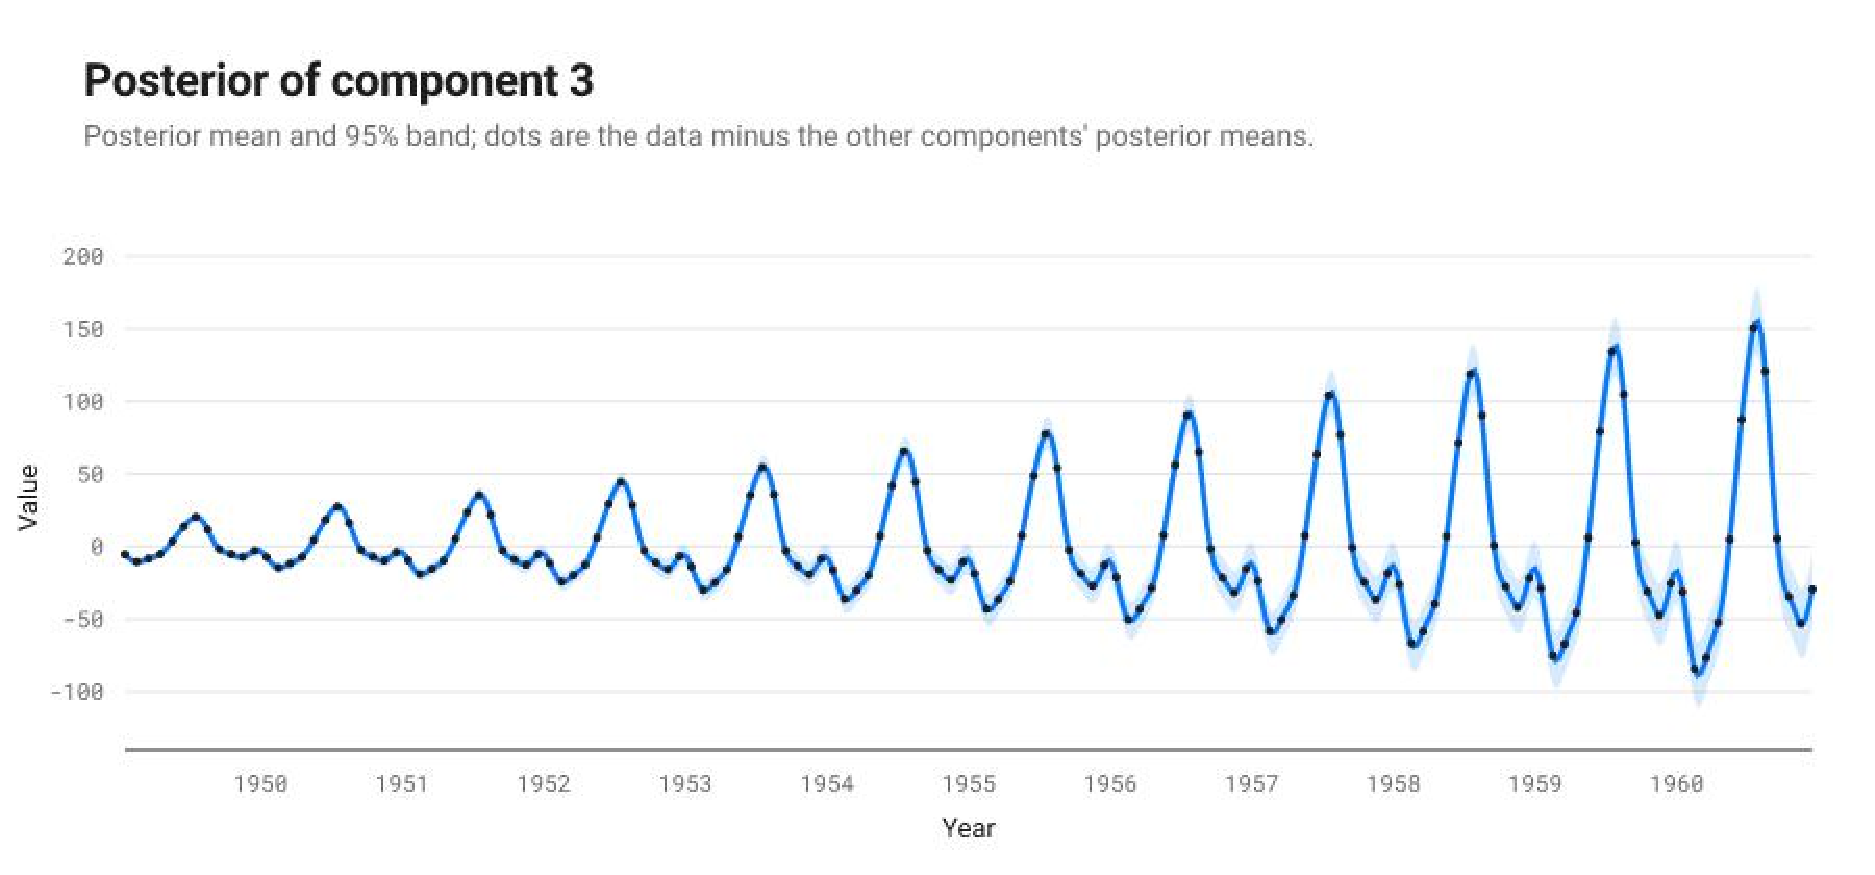
\includegraphics[width=\linewidth]{component_3.pdf}
\caption*{Component 3}
\end{figure}
\subsection*{Component 4: This simple AI is not capable of describing the component Lin x Per x RQ}

This simple AI is not capable of describing the component Lin x Per x RQ.

This component explains -0.8\% of the data's variance on its own; with the components above it, 99.6\%. Adding it changes the cross-validated MAE by -48.1\%.

\emph{Extrapolation.} This simple AI is not capable of describing the component Lin x Per x RQ.

\begin{figure}[H]
\centering
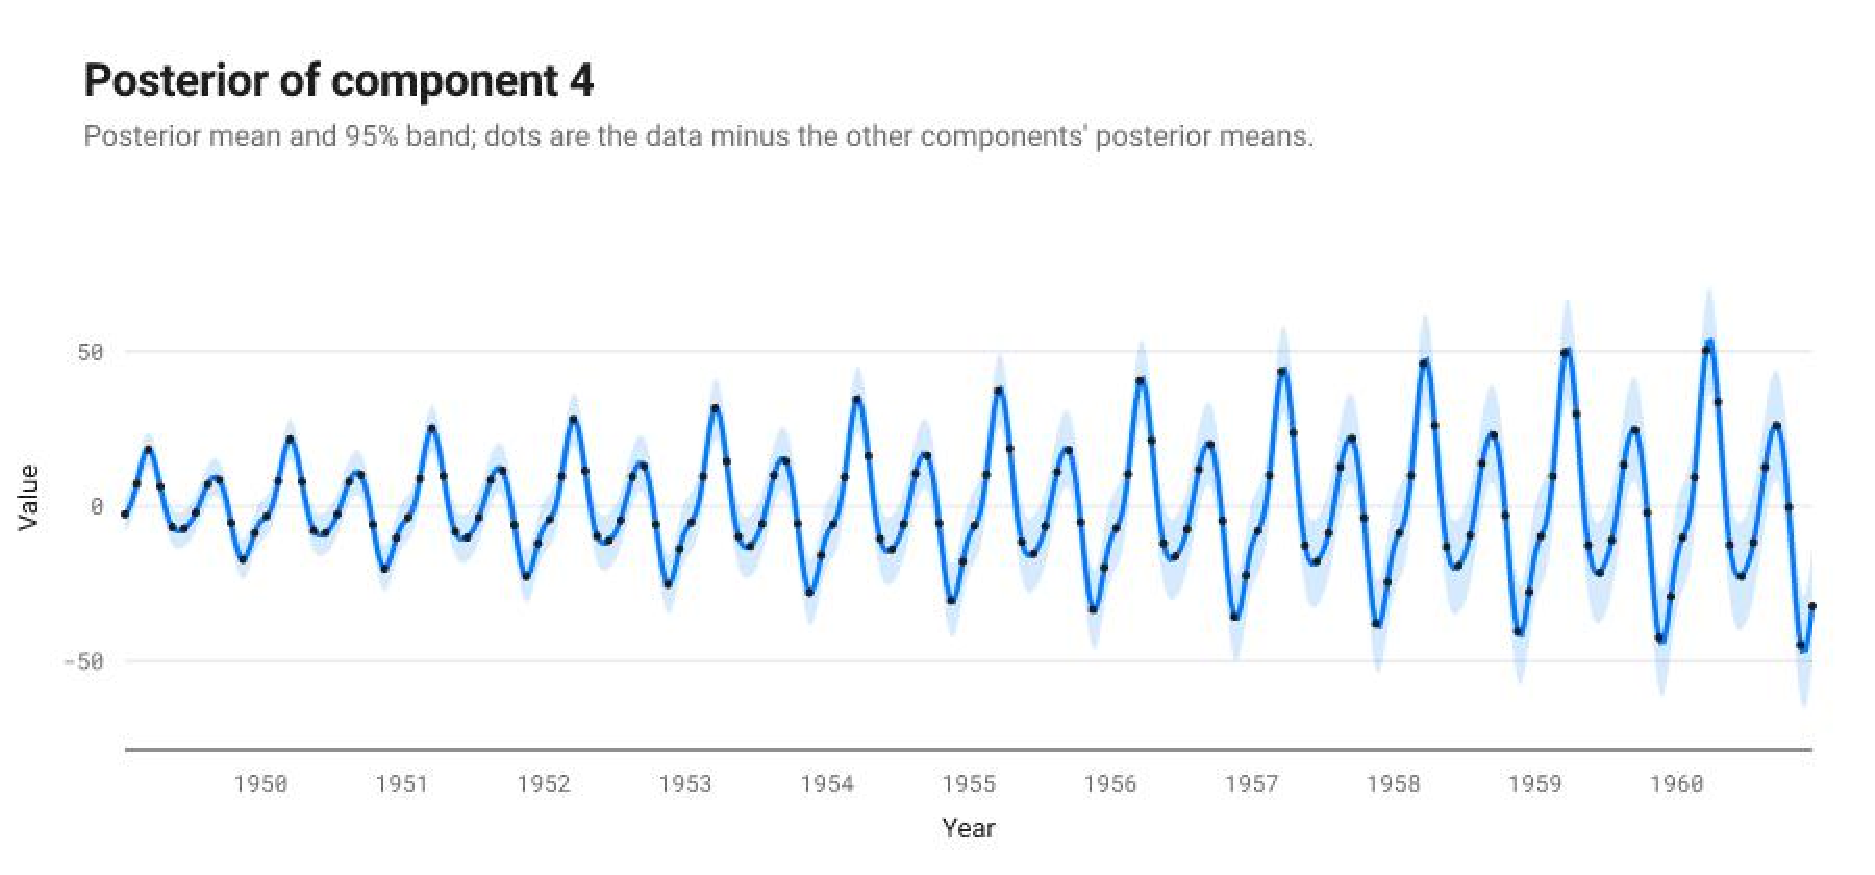
\includegraphics[width=\linewidth]{component_4.pdf}
\caption*{Component 4}
\end{figure}
\subsection*{Component 5: A periodic function with a period of 4.2 years but with linearly increasing amplitude}

This component is periodic with a period of 4.2 years but with varying amplitude. The amplitude of the function increases linearly. The shape of this function within each period has a typical lengthscale of 7.5 months.

This component explains 0.6\% of the data's variance on its own; with the components above it, 100.0\%. Adding it changes the cross-validated MAE by -31.9\%.

\emph{Extrapolation.} This component is assumed to continue periodically with a period of 4.2 years but with varying amplitude. The amplitude of the function is assumed to continue to increase linearly.

\begin{figure}[H]
\centering
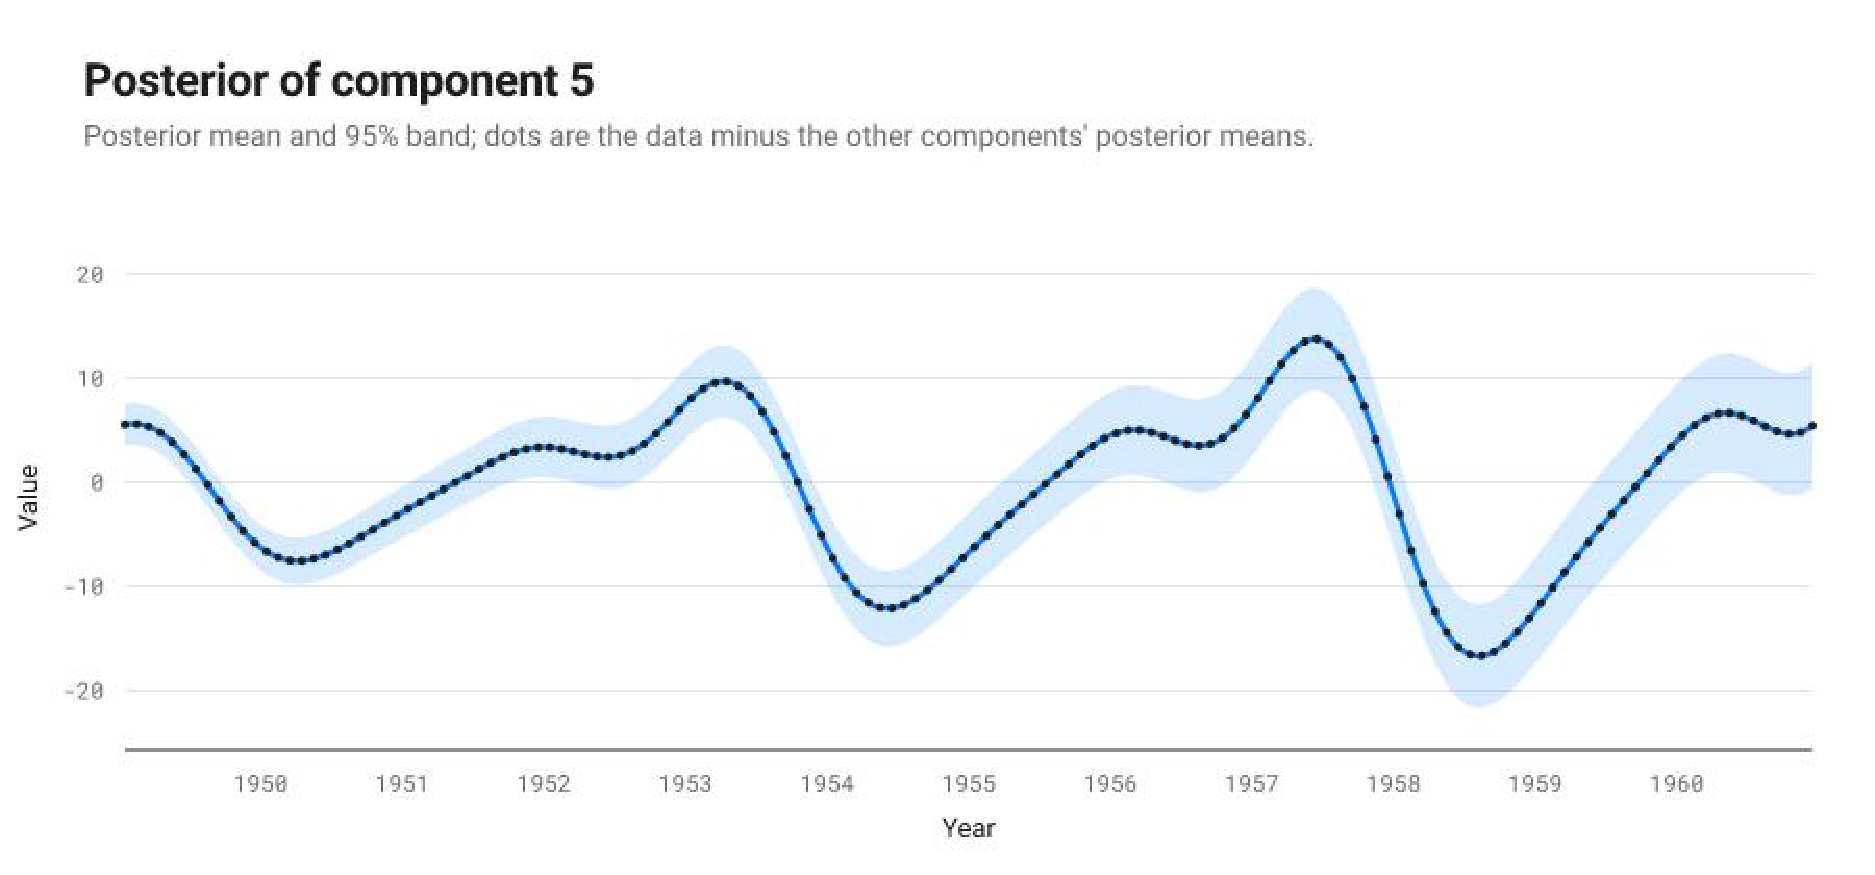
\includegraphics[width=\linewidth]{component_5.pdf}
\caption*{Component 5}
\end{figure}

\section*{Model checking}

Each statistic compares draws of a component's posterior with draws of its prior. A small p-value (bold below 0.05) points at a property of the data that the component's prior does not reproduce.

\begin{center}
\begin{tabular}{lrrrrrrr}
\toprule
\# & QQ max & QQ min & ACF min & ACF min lag & Pgram max & Pgram peak & MMD \\
\midrule
1 & 0.284 & 0.284 & 0.982 & 0.988 & 0.564 & 0.974 & \textbf{0.000} \\
2 & 0.324 & 0.344 & 0.496 & 0.774 & 0.672 & 0.968 & \textbf{0.000} \\
3 & 0.564 & 0.272 & 0.784 & 0.824 & 0.522 & 0.638 & 0.087 \\
4 & 0.958 & 0.580 & 0.770 & 0.554 & 0.904 & 0.412 & \textbf{0.016} \\
5 & 0.424 & 0.848 & 0.824 & 0.792 & 0.964 & 0.682 & \textbf{0.003} \\
\bottomrule
\end{tabular}
\end{center}

QQ: quantile-quantile gaps. ACF: autocorrelation function. Pgram: periodogram. MMD: maximum mean discrepancy two-sample test.

\end{document}
